%%%%%%%%%%%%%%%%%%%%%%%%%%%%%%%%%%%%%%%%%
% Stylish Article
% LaTeX Template
% Version 1.0 (31/1/13)
%
% This template has been downloaded from:
% http://www.LaTeXTemplates.com
%
% Original author:
% Mathias Legrand (legrand.mathias@gmail.com)
%
% License:
% CC BY-NC-SA 3.0 (http://creativecommons.org/licenses/by-nc-sa/3.0/)
%
%%%%%%%%%%%%%%%%%%%%%%%%%%%%%%%%%%%%%%%%%

%----------------------------------------------------------------------------------------
%	PACKAGES AND OTHER DOCUMENT CONFIGURATIONS
%----------------------------------------------------------------------------------------

\documentclass[fleqn]{SelfArx} % Document font size and equations flushed left

\definecolor{color1}{RGB}{0,0,90} % Color of the article title and sections
\definecolor{color2}{RGB}{0,20,20} % Color of the boxes behind the abstract and headings

\newlength{\tocsep} 
\setlength\tocsep{1.5pc} % Sets the indentation of the sections in the table of contents
\setcounter{tocdepth}{3} % Show only three levels in the table of contents section: sections, subsections and subsubsections

\usepackage{lipsum} % Required to insert dummy text
\usepackage{mathrsfs}
%----------------------------------------------------------------------------------------
%	ARTICLE INFORMATION
%----------------------------------------------------------------------------------------

\JournalInfo{10-701} % Journal information
\Archive{Machine Learning} % Additional notes (e.g. copyright, DOI, review/research article)

\PaperTitle{Autonomous Visualization for Unsupervised Learning (Final Report)} % Article title

\Authors{Yun Ni(yunn), Yang Lu(yanglu2), Zhangning Hu(zhangnih)} % Authors

\Keywords{Data Visualization---Unsupervised Learning---Hartigan's Dip Test---Minimum Spanning Tree---Clustering} % Keywords - if you don't want any simply remove all the text between the curly brackets
\newcommand{\keywordname}{Keywords} % Defines the keywords heading name

%----------------------------------------------------------------------------------------
%	ABSTRACT
%----------------------------------------------------------------------------------------

\Abstract{Visualization of high-dimensional data is critical to data analysis and can be helpful to extract insights from multidimensional data sets. However, it is difficult to visualize high-dimensional clusters because clustering results often suffer from a lack of human interpretability. In this project, we explore effective techniques that autonomously discovers patterns in high-dimensional unlabeled data and visualize it in form of two-dimensional scatter plots with interpretable axes. We discover the best scatter plot by finding potential multimodal distributions using two approaches: Hartigan's Dip Test and Minimum Spanning Tree. We will compare the results of these two methods in our final report.}

%----------------------------------------------------------------------------------------

\begin{document}

\flushbottom % Makes all text pages the same height

\maketitle % Print the title and abstract box

%\tableofcontents % Print the contents section

\thispagestyle{empty} % Removes page numbering from the first page

%----------------------------------------------------------------------------------------
%	ARTICLE CONTENTS
%----------------------------------------------------------------------------------------

\section{Introduction} % The \section*{} command stops section numbering

\addcontentsline{toc}{section}{\hspace*{-\tocsep}Introduction} % Adds this section to the table of contents with negative horizontal space equal to the indent for the numbered sections

Many machine learning algorithms suffer from a lack of human interpretability. As a result, many domain experts find it difficult to adopt machine learning techniques. With the growing inter-discipline research, the interpretability of classification and clustering is becoming more essential.\\

\cite{av} present a novel approach to classification that takes into account visualization of the results. Concretely, the authors have suggested a way to efficiently discover the most relevant snapshot of the data, in the form of a two-dimensional scatter plot with easily understandable axes.\\

In this project, we are making similar approach to the visualization of clustering. However, we search a much larger expression space and we suggest our own way to define and calculate the "interpretability" of scatter plot.

%------------------------------------------------
\section{Related Works}
\section{Problem Definition}
More formally, given a dataset ${d_1 , d_2\cdots d_m }$, we want to search the function space $F: D \rightarrow R^2$
for the optimal function

$$\arg\max_{f \in F} Pr\{f(d_1), f(d_2),\cdots f(d_m)\ is\ multimodal\ distributed\}$$

so that we can easily see the clusters by scatter-plotting $f(d_1), f(d_2),\cdots f(d_m)$.\\
\\

Ideally, the function space F should be all the functions that are interpretable by humans. But to simplified the problem, we limit our functions to include at most 4 attributes in the dataset. That means
we search over all the quadraple of the attributes and find the optimal function $f*$.

\section{Methodology}

Our project involves answering the following questions:
\begin{itemize}
\item[1.] How can we define and calculate the "interpretability" of a scatter plot?
\item[2.] How can we find the pair of expressions with best "interpretability"? 
\end{itemize}

\subsection{Expression Search}

We will answer question 2 first. Assume we have already implement the calculation of the interpreterability score, we want to find the optimal scatter plot. As mentioned above, for the sake of interpreterability, we limit the number of attributes we use to be at most 4.\\

Let $n$ be the number of attributes, $u$ be the number of unary operations and $b$ be the number of binary operations. If we search every quadruple of variables, it would take $O((un)^4b^2)$, which is computationally infeasible.\\

Rather than exhaustively searching all possible x-expression and y-expression. We use greedy search to find an approximation of the best pair of expressions:

\begin{itemize}
\item[1.] We exhaustively search all pairs of attributes with unary operations, recording the best pair.
\item[2.] Given the best pair, we consider all triples that contain the best pair, recording the best pair.
\item[3.] Given the best triple, we consider all quadruples that contain the best triple, recording the best pair.
\item[4.] We try to add unary operation to either expression. output the best pair.
\end{itemize}

The intuition behind this search is that if scatter plot $(op(x), y)$ is the best scatter plot, then scatter plot $(x, y)$ is also a very good scatter plot.\\

Using the fast expression search algorithms, it takes $O((un)^2 + 2bun)=O(b(un)^2)$ to find the optimal scatter plot.
\subsection{Scoring Scatter Plot}
\subsubsection{Hartigan's Dip Test}


In this project, we will test three interpretability scores. The first is Hartigan's Dip Test. In\cite{dip}, J.A. Hartigan and P.M. Hartigan introduces the dip test which test a one-dimensional distribution function's unimodality. The dip is defined as following: Let $\rho(f,g)=sup_x|f(x)-g(x)|$ for bounded functions $f,g$. Let  $\rho(f,\mathscr{A})=inf_{g\in \mathscr{A}}|f(x)-g(x)|$, where $\mathscr{A}$ is a set of bounded functions. Let $\mathscr{U}$ denotes the set of unimodal distribution functions. The dip is defined as:
\begin{equation}
D(f)=\rho (f, \mathscr{U})
\end{equation}

So the dip is a measure of distance of a distribution function from its best fit unimodal distribution. We use dip as the base of our interpretability score to test clustering structure in scatter plots we get. The intuition is that if the data points have a structure of more than one cluster, its distribution function will be multimodal which is "far away" for the set of unimodal distribution functions. Therefore it will have a large dip.\\

Notice that dip test detects multimodality of one-dimensional distribution functions. However, our scatter plots are two-dimensional. J.A. Hartigan and M. Rozal introduces in \cite{MAP} the MAP test which detects multimodal in multi-dimensional distributions based on Minmum Spanning Tree. We will discuss it in next section. \\

\begin{figure}[h]
  \centering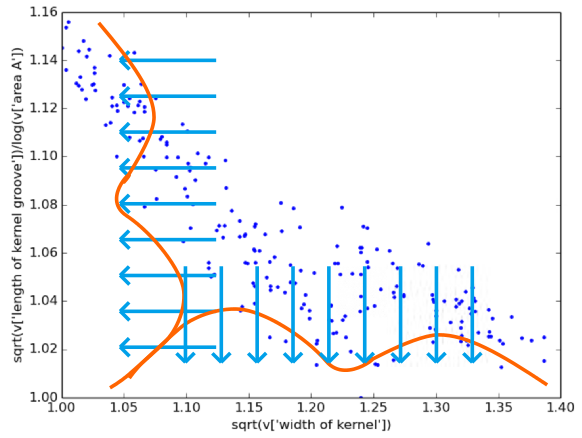
\includegraphics[width=0.5\textwidth]{HDT}
  \caption{Project the data and calculate the sum of the dip}
\end{figure}

Here we use a staightforward method. We project the plots to x and y axis to get two one-dimensional distributions. Then we use the sum of dips of those two distributions as the score of interpretability. This straightforward method works pretty well as shown in our result. 

\subsubsection{Modes Distance}
Another approach to score scatter plot is the modes distance. Concretely, we use a moving window to scan over the scatter plot. Within each window, we compute the number of points inside. Having the number of points in each window, we then compute the distance between the top two windows (in fraction of the plot
size) as the score of the scatter plot.\\

\begin{figure}[h]
  \centering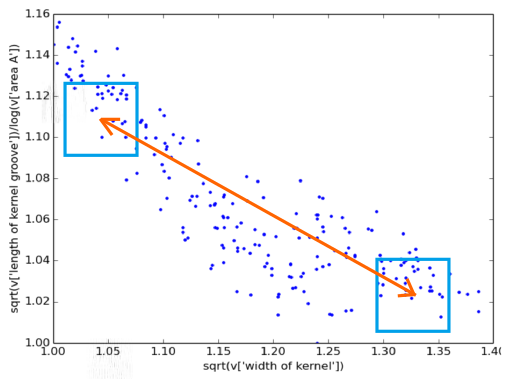
\includegraphics[width=0.5\textwidth]{window}
  \caption{Minimum Spanning Tree contains the potential clusters}
\end{figure}

The intuition behind this scoring method is that clusters far away from each other tends to be more 'interpretable'. If there is only one cluster in the scatter plot, the top two windows are likely to be very close to each other because they belong to the same cluster. If there are multiple clusters, the top two windows probably belong to different clusters so that the distance between them is longer than the previous case.

\subsubsection{Partial Minimum Spanning Tree}

Intuitively, the third interpretability score we will try is to build a partial minimum spanning tree on the scatter plot. The advantage of building a Minimum Spanning Tree is that it contains the structure of the scatter plot. Thus based on MST, we can decide whether the structure is interpretable or not.\\

\begin{figure}[h]
  \centering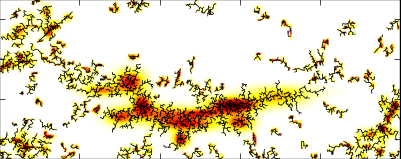
\includegraphics[width=0.7\textwidth]{fig_great_wall_MST_1}
  \caption{Minimum Spanning Tree contains the potential clusters}
\end{figure}

Minimum Spanning Tree is usually built based a graph. It is computational infeasible if we build a clique including all possible edges, and then run Borůvka's algorithm, Prim's algorithm, or Kruskal's algorithm to find the minimum spanning tree. Ideally, we want the algorithm to run in $O(nlogn)$ time so we can do a fast search over all possible expressions.\\

So how can we design a feasible algorithm to build Minimum Spanning Trees in Euclidean space? The answer is Delaunay triangulations.\\

Delaunay triangulations maximize the minimum angle of all the angles of the triangles in the triangulation; they tend to avoid skinny triangles.\cite{tra} Because the Delaunay triangulation is a planar graph, and there are no more than three times as many edges as vertices in any planar graph, this generates only $O(n)$ edges. With $O(n)$ edges, we are able to build Minimum Spanning Tree in $O(nlogn)$.\cite{mst}\\

\begin{center}
\begin{figure}[h]
  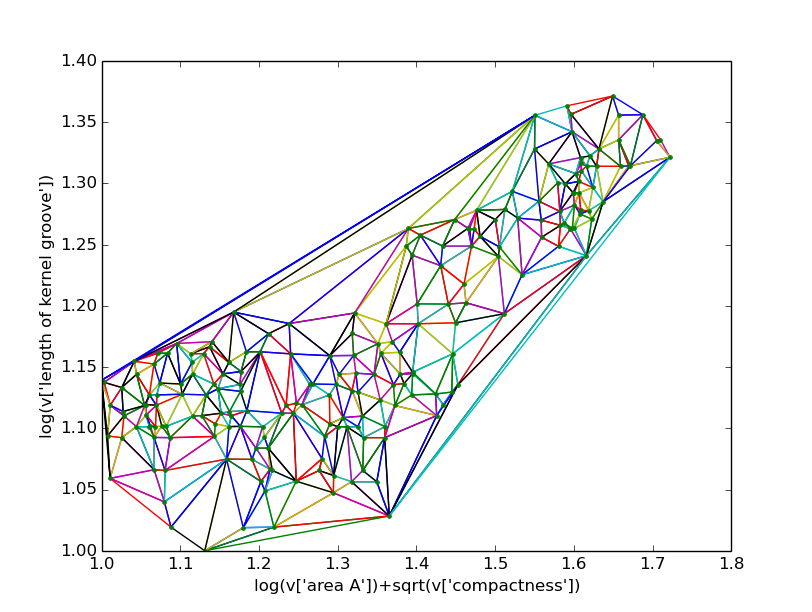
\includegraphics[width=0.45\textwidth]{figure_1}
  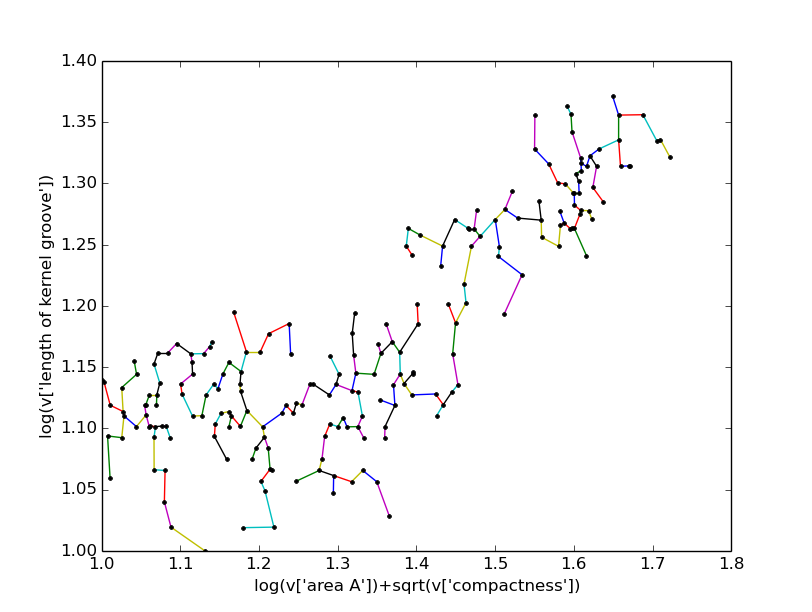
\includegraphics[width=0.45\textwidth]{figure_2}
  \caption{Building MST in Euclidean Space. Left: Delaunay Triangulation; Right: Minimum Spanning Tree.}
\end{figure}
\end{center}

After we build the minimum spanning tree, we need to define a score based on it. Intuitively, the edges connecting vertices within a cluster tend to be short, while the edges connecting vertices between different clusters have larger weights. As a result, we build only a part of the minimum spanning tree where all edges are smaller than a threshold $\lambda$. This is what we called "Partial Minimum Spanning Tree".\\

Assume $k$ clusters are of the same size and the same dense. If there is only one cluster, then there tends to be a big connected component in the partial minimum spanning tree. If the number of clusters is $k$, then the top $k$ connected components are likely to be equal in size. As a result, we use the size of the second largest component as an indicator of how likely there are more than one cluster. \\

\begin{figure}[h]
  \centering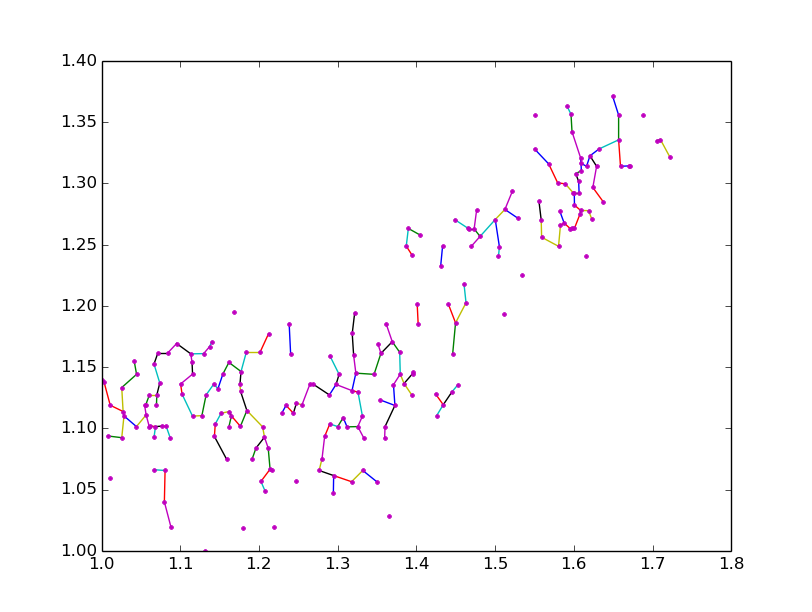
\includegraphics[width=0.5\textwidth]{figure_3}
  \caption{Partial Minimum Spanning Tree: Include edges no longer than $\lambda$}
\end{figure}

To summarize, we follow these steps to calculate score for a scatter plot:
\begin{itemize}
\item[1.] Use Delaunay triangulation to build a graph
\item[2.] Run Kruskal's algorithm to build our Minimum Spanning Tree
\item[3.] Exclude all the edges longer than $\lambda$
\item[4.] Output the number of vertices in the second largest connected component as the score.
\end{itemize}

\section{Experiments}

\subsection{Dataset \& Expression Space}
The Dataset we use in our project is the Seeds Data Set from UCI Machine Learning Repository. Each instance in the dataset stands for one type of seed. The information are collected on three kind of seeds: Kama, Rosa and Canadian. However, no instance is labelled so that the dataset can be used to test clustering.\\

To construct the data, seven geometric parameters of wheat kernels were measured: 
\begin{itemize}
\item area A, 
\item perimeter P, 
\item compactness $C = 4\times pi\times A/P^2$, 
\item length of kernel, 
\item width of kernel, 
\item asymmetry coefficient 
\item length of kernel groove. 
\end{itemize}
All of these parameters were real-valued continuous.\\

We search a wide range of expressions connecting the parameters above by a number of unary and binary operators. The unary and binary operators we use in our project are:

$$unary = [log, exp, sqrt]$$
$$binary = [+, -, *, /, **]$$

\subsection{Results}

\subsubsection{Hartigan's Dip Test}

Hartigan's dip test scoring method has achieved interesting result in the first dataset. In Figure 6, our algorithm pick $compactness^{areas}$ as x-axis and $len\_groove$ as y-axis. We can clearly see two clusters, and the third cluster is on right of the down-left cluster. By contrast, we plot the $(compactness, len\_groove)$ without operations. We find it difficult to tell any of the clusters.\\

\begin{center}
\begin{figure}[h]
  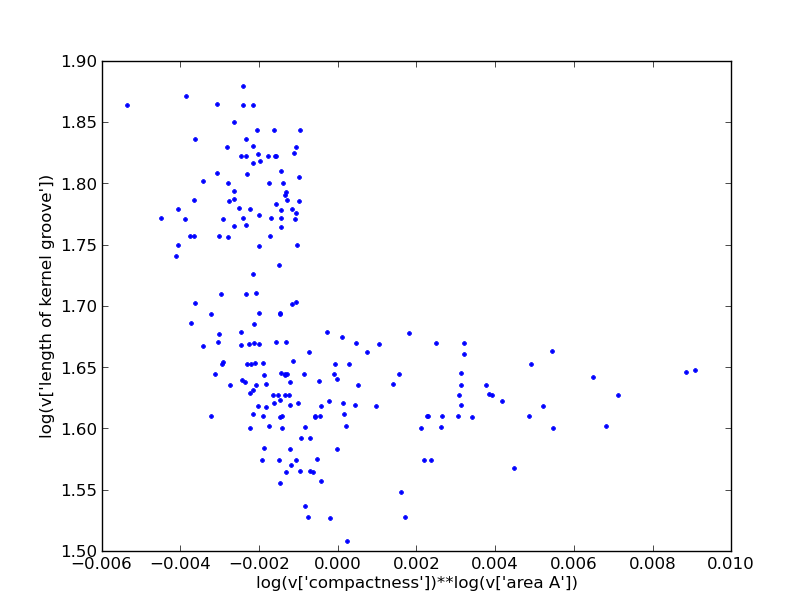
\includegraphics[width=0.45\textwidth]{Seed}
  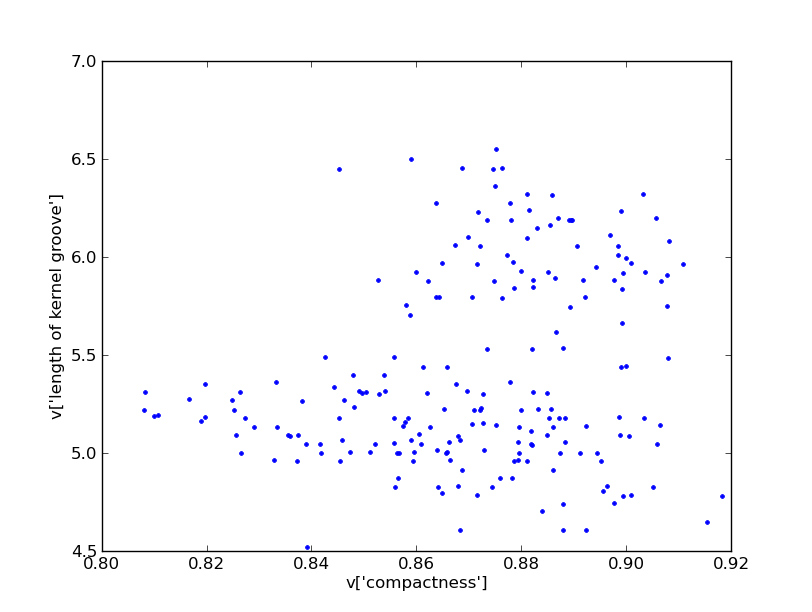
\includegraphics[width=0.45\textwidth]{seed_before}
  \caption{The left is the best scatter plot we find. The right is for contrast.}
\end{figure}
\end{center}

We also can know more about the shortcoming of this score method. It can only find clusters parallel to x-axis or y-axis, which limits the position of the cluster we can interpret.

\subsubsection{Modes Distance}
Compared to Hartigan's Dip Test, Modes Distance did not achieved very good result. We have tried with different window sizes and different offsets. The best scatter plot we can find is $\sqrt{width\_kernel}$ vs $\sqrt{len\_groove}/{areas}$. It has two dense windows on the up-left and down-write, which maximize the modes distance. However, the points are actually linearly distributed and the up-left and down-write "clusters" exists because of the noise.

\begin{figure}[h]
  \centering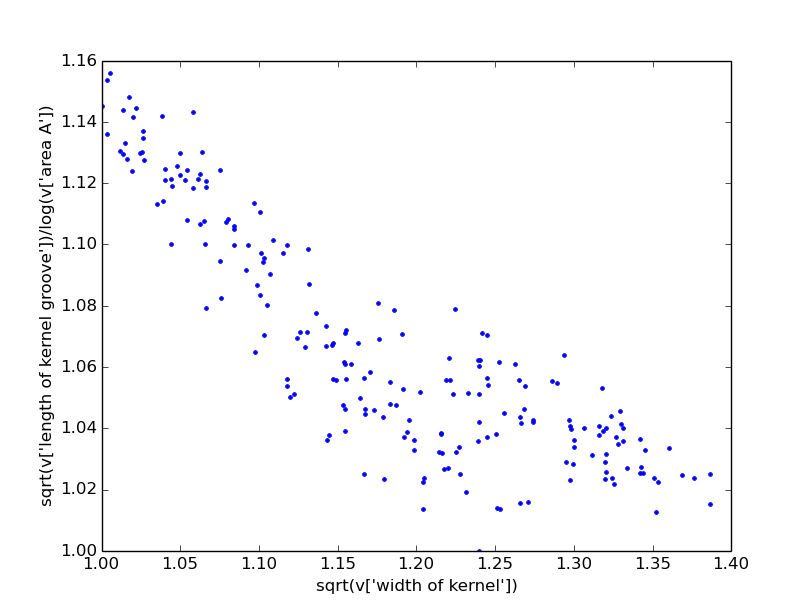
\includegraphics[width=0.5\textwidth]{distance}
  \caption{Best Scatter Plot found by Modes Distance}
\end{figure}

\subsubsection{Partial Minimum Spanning Tree}
The 3rd scoring metric also brings interesting results. Instead of finding 3 clusters in Hartigan's Dip Test, it finds 2 clusters, but not parallel to x-axis or y-axis. Moreover, the expressions of x-axis and y-axis are much more simpler than that of Hartigan's Dip Test. We can interpret the clusters plotting by $(width\_kernel, exp(len\_groove))$ very easily.

\begin{figure}[h]
  \centering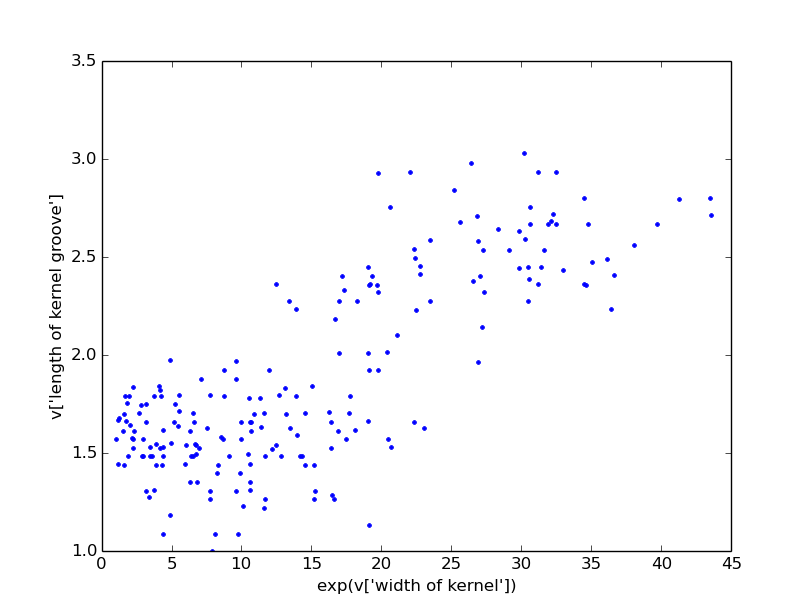
\includegraphics[width=0.5\textwidth]{mst}
  \caption{Best Scatter Plot found by Partial Minimum Spanning Tree}
\end{figure}

\section{Conclusion}

%------------------------------------------------

%----------------------------------------------------------------------------------------
%	REFERENCE LIST
%----------------------------------------------------------------------------------------

\bibliographystyle{unsrt}
\bibliography{reference}

%----------------------------------------------------------------------------------------

\end{document}